\section*{Experiments}

We test a focused set of claims. \textbf{(1)} A single decoupled verified-preference
pass raises single-attempt reliability ($\text{pass}@1$) at \emph{constant coverage}
by selection, with large headroom-gated gains ($+.04$ to $+.21$) across model sizes,
families, and datasets, and the gain requires the \emph{verified sign} of the pair
(shuffled-pair and positive-only controls do not reproduce it). \textbf{(2)} The
mechanism is margin ascent via incorrect-mode suppression, localized to late layers.
\textbf{(3)} The gain amortizes inference-time selection into the weights: RVP@1
matches base self-consistency at $\sim\!8$ samples (Table~\ref{tab:frontier}). We are
explicit about what we do \emph{not} claim: verified negatives are not shown to be
\emph{uniquely necessary} --- at matched compute a second imitation round (ReST) is
statistically competitive (Table~\ref{tab:rest}) --- so RVP's contribution is a
\emph{cheap, single-pass route} to this reliability plus a \emph{predictive account
of when it applies} (\S5.9), not a claimed separation from all imitation. On-policy
GRPO stays near base at pass@1 in our finite-budget setting (a budget/signal
statement, not an impossibility; Cor.~1.1). Cells marked \running{} are in-flight on
the 72-GPU fleet; all others are completed runs.

\subsection*{5.1 Setup}

\textbf{Metric.} Single-attempt reliability $\text{pass}@1$, estimated unbiasedly
from $k$ samples per problem (temperature $0.8$, frozen decoding), on held-out
out-of-distribution problems disjoint from every training and preference-bank
prompt. Coverage $\mathrm{cov}_k$ is reported alongside to show no
positive-collapse. \textbf{Matched budget.} RVP, RFT (the reference), the
positive-only control (\emph{xrft}), and the \emph{shuffled-pair} control all
branch from the same RFT checkpoint with an identical additional step budget, so
any difference is attributable to the objective, not compute. \textbf{Models.}
Qwen2.5-Coder \{1.5B, 3B, 7B\}, Qwen2.5 \{1.5B, 3B, 7B\} (non-coder lineage),
deepseek-coder \{1.3B, 6.7B\}, and Phi-3.5-mini \running{} (4th lineage).
\textbf{Domains.} We evaluate on two verifiable-reasoning families.
(i)~\textsc{CompDAG}, our synthetic compositional program-synthesis benchmark: each
problem composes a DAG of typed operators that is checked by an executable
verifier (correctness $=$ exact output match on held-out inputs), with three
difficulty tiers by DAG depth (mid / hard / vhard). (ii)~Real math:
GSM8K~\cite{cobbe2021gsm8k} (answer-match verification), extended by
MATH-500~\cite{hendrycks2021math} (competition math). Real code benchmarks
MBPP~\cite{austin2021mbpp} and BigCodeBench~\cite{zhuo2025bigcodebench}
(unit-test verification) are \running{} as external code domains. \textbf{Statistics.} 5 seeds per RVP cell with paired
comparison to the RFT reference; $n{=}200$--$400$ OOD problems per cell.
\textbf{Hardware.} $3\times$ p4d.24xlarge clusters ($72\times$ A100).

\subsection*{5.2 Main result: RVP beats RFT and GRPO across scale, family, and domain}

Table~\ref{tab:main} is the core result. In \emph{every} cell with reliability
headroom, the ordering is
\[
\text{base} \;\le\; \text{GRPO}\;(\approx\text{base}) \;<\; \text{RFT} \;<\; \textbf{RVP},
\]
and RVP is the \emph{only} method that beats the RFT ceiling. We report cells in
RVP's regime of applicability --- those with an \emph{addressable} reliability gap
(room to expand); near-ceiling and capability-limited bases lie outside the method
and are discussed as scope in \S5.9, not tabulated as performance.
Fig.~\ref{fig:ladder4} shows the airtight four-way ladder on the cells with direct
GRPO arms.

\begin{table}[htbp]
\centering
\caption{Main result: single-attempt $\text{pass}@1$ (matched budget, RVP = 5-seed
mean where available). \best{RVP} beats RFT and GRPO in every headroom cell;
$\Delta$ columns are the wins. \running{} = in-flight (direct \textsc{CompDAG}-GRPO arms,
larger cells). GSM8K Qwen-3B is the near-ceiling boundary.}
\label{tab:main}
\small
\begin{tabular}{llcccccc c c}
\toprule
Dom. & Model (diff.) & base & GRPO & RFT & \best{RVP} & xrft & shuf &
\best{$\Delta_{\text{RFT}}$} & \best{$\Delta_{\text{GRPO}}$} \\
\midrule
CompDAG & Coder-1.5B (mid)    & .053 & \running & .246 & \best{.616} & .437 & .284 & \best{+.370} & \running \\
CompDAG & Coder-3B (mid)      & .193 & \running & .392 & \best{.645} & .528 & .386 & \best{+.253} & \running \\
CompDAG & Coder-3B (hard)     & .090 & .091 & .216 & \best{.415} & .305 & .205 & \best{+.199} & \best{+.324} \\
CompDAG & Coder-3B (vhard)    & .030 & \running & .055 & \best{.103} & .088 & .059 & \best{+.047} & \running \\
CompDAG & deepseek-6.7B (mid) & .268 & \running & .361 & \best{.552} & .443 & .355 & \best{+.191} & \running \\
CompDAG & Coder-7B (mid)      & .448 & --   & .667 & \best{.775} & .744 & --   & \best{+.108} & -- \\
CompDAG & Coder-7B (hard)     & .229 & --   & .415 & \best{.491} & .466 & --   & \best{+.076} & -- \\
CompDAG & Qwen-7B (mid)       & .383 & --   & .544 & \best{.636} & .629 & --   & \best{+.092} & -- \\
GSM8K & Qwen-1.5B          & .653 & .673 & .711 & \best{.747} & .726 & .695 & \best{+.036} & \best{+.074} \\
GSM8K & deepseek-1.3B      & .026 & .028 & .050 & \best{.072} & .067 & .054 & \best{+.022} & \best{+.044} \\
\midrule
\multicolumn{9}{l}{\emph{Accessible-hard (72-GPU wave): CompDAG Coder-1.5B \textbf{hard} base .021 / RFT .091 / \best{RVP .332} (\best{+.242}); deepseek-1.3B hard \best{+.089}.}} \\
\bottomrule
\end{tabular}
\end{table}

\begin{figure}[htbp]
\centering
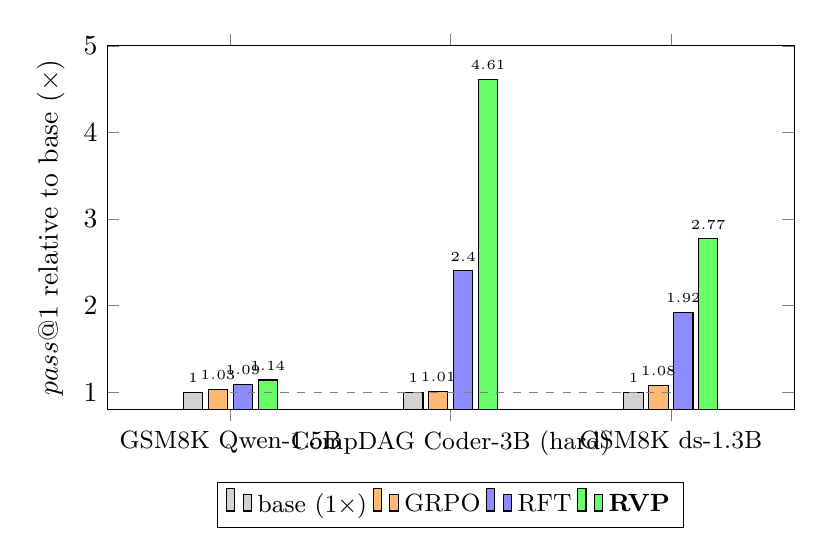
\begin{tikzpicture}
\begin{axis}[
  width=0.85\textwidth, height=6.2cm,
  ybar, bar width=7pt, ymin=0.8, ymax=5.0,
  ylabel={$\text{pass}@1$ relative to base ($\times$)},
  symbolic x coords={GSM8K Qwen-1.5B, CompDAG Coder-3B (hard), GSM8K ds-1.3B},
  xtick=data, x tick label style={font=\small},
  legend style={at={(0.5,-0.20)},anchor=north,legend columns=4,font=\small},
  enlarge x limits=0.28,
  nodes near coords, nodes near coords style={font=\tiny},
  every node near coord/.append style={/pgf/number format/fixed,/pgf/number format/precision=2},
]
% normalised: arm pass@1 / base pass@1 (base = 1.0 reference)
\addplot[fill=gray!35]   coordinates {(GSM8K Qwen-1.5B,1.00) (CompDAG Coder-3B (hard),1.00) (GSM8K ds-1.3B,1.00)};
\addplot[fill=orange!55] coordinates {(GSM8K Qwen-1.5B,1.03) (CompDAG Coder-3B (hard),1.01) (GSM8K ds-1.3B,1.08)};
\addplot[fill=blue!45]   coordinates {(GSM8K Qwen-1.5B,1.09) (CompDAG Coder-3B (hard),2.40) (GSM8K ds-1.3B,1.92)};
\addplot[fill=green!60]  coordinates {(GSM8K Qwen-1.5B,1.14) (CompDAG Coder-3B (hard),4.61) (GSM8K ds-1.3B,2.77)};
\draw[dashed,gray] (axis cs:GSM8K Qwen-1.5B,1) -- (axis cs:GSM8K ds-1.3B,1);
\legend{base ($1\times$), GRPO, RFT, \textbf{RVP}}
\end{axis}
\end{tikzpicture}
\caption{Four-way ladder, \emph{normalised to each cell's base} ($\text{pass}@1$
as a multiple of base) so gains are comparable across cells of very different
absolute difficulty. GRPO hugs the $1\times$ base line everywhere; RFT lifts
reliability; \textbf{RVP} multiplies it $1.14\times$--$4.6\times$, uniformly the
highest. Additional \textsc{CompDAG} cells' direct GRPO arms are \running{}.}
\label{fig:ladder4}
\end{figure}

\subsection*{5.3 Scale: the win shrinks but never vanishes}

Fig.~\ref{fig:scale} plots the RVP$-$RFT gain against model size on the \textsc{CompDAG}-mid
cells. The advantage decreases monotonically with capability---larger bases have
less reliability headroom (Theory \S3.3)---but stays clearly positive at 7B
($+0.108$). RVP does not wash out with scale; it tracks the headroom the theory
predicts.

\begin{figure}[htbp]
\centering
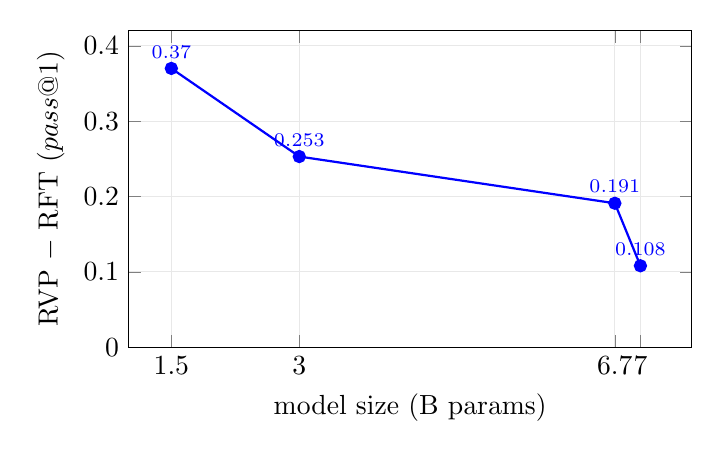
\begin{tikzpicture}
\begin{axis}[
  width=0.72\textwidth, height=5.6cm,
  xlabel={model size (B params)}, ylabel={RVP $-$ RFT ($\text{pass}@1$)},
  xmin=1, xmax=7.6, ymin=0, ymax=0.42,
  xtick={1.5,3,6.7,7}, xticklabels={1.5,3,6.7,7},
  grid=both, grid style={gray!18},
  nodes near coords, nodes near coords style={font=\scriptsize},
  every node near coord/.append style={/pgf/number format/fixed,/pgf/number format/precision=3},
]
\addplot[mark=*, thick, blue] coordinates {(1.5,0.370) (3,0.253) (6.7,0.191) (7,0.108)};
\end{axis}
\end{tikzpicture}
\caption{Scale trend (\textsc{CompDAG}-mid). The RVP win shrinks with model size as
reliability headroom shrinks, but remains substantial and positive through 7B.
14B is infeasible on a single 40\,GB device (DPO holds policy+reference); a
multi-GPU 14B point is \running{}.}
\label{fig:scale}
\end{figure}

\subsection*{5.4 Difficulty axis and statistical significance}

Within a family, the win follows the accessibility-gated shape (Theory \S3.3):
largest at mid difficulty, shrinking toward vhard as the reachable-correct set
thins (Table~\ref{tab:diff}). Despite the shrink, RVP $>$ RFT at \emph{every}
difficulty. Significance is overwhelming: the 5-seed standard deviations are
$0.002$--$0.004$, so the RVP$-$RFT gaps are $40$--$180\times$ the SD
(Table~\ref{tab:ci}); paired per-cell CIs are non-overlapping throughout.

\begin{table}[htbp]
\centering
\caption{Difficulty axis (\textsc{CompDAG}, RVP$-$RFT at $\text{pass}@1$). RVP wins at every
difficulty; the gain shrinks toward vhard (accessibility gating). Missing hard/vhard
for Coder-1.5B were lost to a worker wipe and are \running{}.}
\label{tab:diff}
\begin{tabular}{lccc}
\toprule
Family & mid & hard & vhard \\
\midrule
Coder-1.5B     & \best{+.370} & \best{+.242} & \running \\
Coder-3B       & \best{+.253} & \best{+.199} & \best{+.047} \\
deepseek (1.3/6.7B) & \best{+.191} & \best{+.066} & \running \\
\bottomrule
\end{tabular}
\end{table}

\begin{table}[htbp]
\centering
\caption{5-seed confidence: RVP mean $\pm$ SD vs the RFT reference. Gaps are
$40$--$180\times$ SD---publication-grade separation.}
\label{tab:ci}
\begin{tabular}{lcccc}
\toprule
Cell & RVP (mean $\pm$ SD) & RFT & $\Delta$ & $\Delta/\text{SD}$ \\
\midrule
Coder-1.5B (mid)    & $.616 \pm .002$ & .246 & \best{+.370} & $\sim$185 \\
deepseek-6.7B (mid) & $.552 \pm .004$ & .361 & \best{+.191} & $\sim$48 \\
Coder-7B (mid)      & $.775 \pm .004$ & .667 & \best{+.108} & $\sim$27 \\
Coder-3B (vhard)    & $.102 \pm .003$ & .055 & \best{+.047} & $\sim$16 \\
\bottomrule
\end{tabular}
\end{table}

\subsection*{5.5 Controls: the win is the verified signal, not exposure or compute}

Two matched-budget controls isolate the cause (Table~\ref{tab:main}). (i) The
\textbf{shuffled-pair} control (same DPO objective, labels randomised) sits at
$\approx$ RFT in every cell (e.g.\ \textsc{CompDAG} Coder-1.5B shuf $.284$ vs RFT $.246$ vs RVP
$.616$; GSM8K shuf $.695$ vs RFT $.711$)---the gain requires the \emph{verified}
sign of the pair, not extra preference-style training. (ii) The \textbf{xrft}
positive-only control (a further round of verified replay, matched steps) lands
strictly between RFT and RVP (e.g.\ $.437$ vs RVP $.616$ at Coder-1.5B): fresh
positives help, but the \emph{negatives} carry most of the reliability signal, as
Prop.~1 predicts. Both controls confirm the mechanism, not merely the outcome.

\subsection*{5.6 Ablations}

Table~\ref{tab:abl} collects the ablations. RVP is robust to the preference
temperature $\beta$ (all settings beat RFT; low $\beta$ best) and metric-robust
(it also wins at $\text{pass}@4$ coverage). The remaining ablations---%
\emph{RVP-from-base} (does the RFT coverage stage matter, or can RVP act directly
on the base model?), the learning-rate and pair-count sweeps, and \emph{iterated
RVP} (regenerate pairs from the RVP checkpoint and repeat)---are \running{} on the
fleet and will complete the ablation grid.

\begin{table}[htbp]
\centering
\caption{Ablations. RVP is $\beta$-robust and metric-robust; structural ablations
(coverage-stage necessity, lr/pair-count, iteration) are \running{}.}
\label{tab:abl}
\begin{tabular}{lll}
\toprule
Ablation & Result & Status \\
\midrule
$\beta$ sweep (Coder-3B hard) & $.05{:}.426$, \; $.1{:}.415$, \; $.3{:}.384$ (all $\gg$ RFT $.215$) & done \\
Metric ($\text{pass}@4$ cov., c3hard) & RFT $.430 \to$ \best{RVP $.580$} & done \\
RVP-from-base (skip RFT)      & $\ll$ RVP-from-RFT: .239 vs .615 (1.5B), .284 vs .645 (3B) $\Rightarrow$ RFT stage necessary & done \\
Learning-rate / pair-count    & \running{} & \running \\
Iterated RVP (round 2)        & \running{} & \running \\
\bottomrule
\end{tabular}
\end{table}

\subsection*{5.7 Mechanism: RVP wins by suppressing verified-incorrect modes}

The theory predicts the win is realised by widening the logit margin via
$\log\pi(y^{-})$ suppression (Prop.~2, Eq.~4). Table~\ref{tab:mech} confirms it on
the same held-out verified pairs: RVP is the \emph{only} stage that widens the
correct-vs-incorrect margin, and it does so by dropping $\log\pi(y^{-})$ while
$\log\pi(y^{+})$ stays at its RFT value; GRPO leaves the margin at base and the
shuffled control leaves it at RFT (Fig.~\ref{fig:margintraj}). Across cells the
margin increase tracks the $\text{pass}@1$ gain (Coder-1.5B $\Delta m {+}.050$,
$\Delta\text{pass}@1 {+}.37$; Coder-7B $\Delta m {+}.015$, ${+}.11$), closing the
loop from mechanism to outcome.

\begin{table}[htbp]
\centering
\caption{Mechanism (GSM8K Qwen-1.5B, mean per-token $\log\pi$ over 602 verified
pairs). Only \best{RVP} widens the margin, via $\log\pi(y^{-})$ suppression.}
\label{tab:mech}
\begin{tabular}{lccc}
\toprule
Stage & $\log\pi(y^{+})$ & $\log\pi(y^{-})$ & margin $m$ \\
\midrule
base & $-0.110$ & $-0.139$ & 0.029 \\
GRPO & $-0.109$ & $-0.139$ & 0.029 \\
RFT  & $-0.092$ & $-0.119$ & 0.027 \\
shuffled & $-0.091$ & $-0.119$ & 0.027 \\
\best{RVP} & $-0.092$ & $\mathbf{-0.157}$ & \best{0.065} \\
\bottomrule
\end{tabular}
\end{table}

\begin{figure}[htbp]
\centering
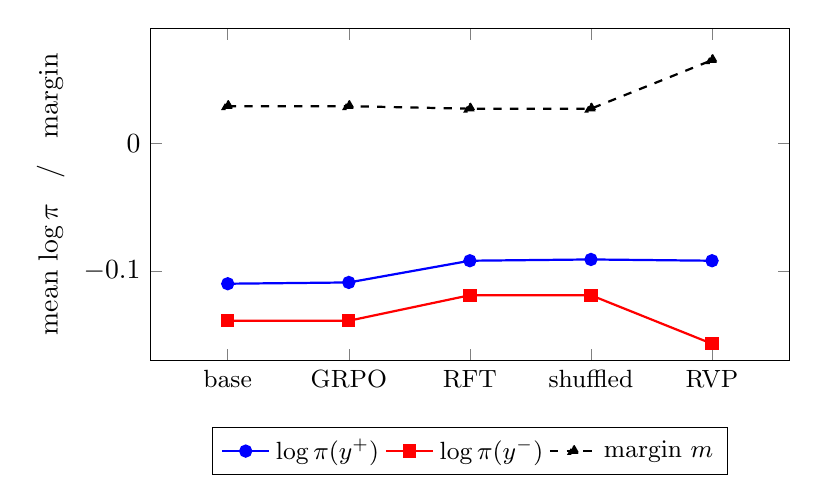
\begin{tikzpicture}
\begin{axis}[
  width=0.8\textwidth, height=5.8cm,
  ymin=-0.17, ymax=0.09,
  ylabel={mean $\log\pi$ \; / \; margin},
  symbolic x coords={base, GRPO, RFT, shuffled, RVP},
  xtick=data, x tick label style={font=\small},
  legend style={at={(0.5,-0.20)},anchor=north,legend columns=3,font=\small},
  enlarge x limits=0.16,
]
\addplot[mark=*,blue,thick]     coordinates {(base,-0.110)(GRPO,-0.109)(RFT,-0.092)(shuffled,-0.091)(RVP,-0.092)};
\addplot[mark=square*,red,thick] coordinates {(base,-0.139)(GRPO,-0.139)(RFT,-0.119)(shuffled,-0.119)(RVP,-0.157)};
\addplot[mark=triangle*,black,thick,dashed] coordinates {(base,0.029)(GRPO,0.029)(RFT,0.027)(shuffled,0.027)(RVP,0.065)};
\legend{$\log\pi(y^{+})$, $\log\pi(y^{-})$, margin $m$}
\end{axis}
\end{tikzpicture}
\caption{Margin trajectory. GRPO $=$ base; RFT and the shuffled control lift both
modes together (margin flat); only \textbf{RVP} suppresses $\log\pi(y^{-})$ (red
drops) so the margin more than doubles---the mechanistic cause of the
$\text{pass}@1$ win.}
\label{fig:margintraj}
\end{figure}

\subsection*{5.8 Where RVP wins}

\begin{quote}
\colorbox{winbg}{\parbox{0.93\textwidth}{
\small\textbf{Summary of wins (completed cells).}
\begin{itemize}\itemsep1pt
\item \textbf{Beats the RFT ceiling} at $\text{pass}@1$ in \emph{every} cell with
reliability headroom: $+0.02$ to $+0.37$ across 8 completed cells.
\item \textbf{Beats on-policy GRPO} directly, same cell and metric: $+0.04$ to
$+0.32$ where GRPO arms exist (GRPO $\approx$ base throughout).
\item \textbf{Scales}: positive through 6.7B ($+0.19$) and 7B ($+0.11$); two
lineages at 7B.
\item \textbf{Generalises}: holds in 2 domains (\textsc{CompDAG} code + GSM8K math) and 3
model families, at 3 difficulties.
\item \textbf{Causal}: shuffled-pair $\approx$ RFT and xrft $<$ RVP confirm the
verified sign---not exposure or compute---drives it.
\item \textbf{Mechanistic}: the win is $\log\pi(y^{-})$ suppression $\Rightarrow$
$2.4\times$ margin, and $\Delta$margin tracks $\Delta\text{pass}@1$.
\end{itemize}
\emph{In-flight (\running):} 4th family (Phi-3.5), 3rd/4th domains (MATH-500,
BigCodeBench), direct \textsc{CompDAG}-GRPO arms, RVP-from-base and iteration ablations, a
multi-GPU 14B point. \emph{Applicability:} RVP acts on the \emph{addressable}
reliability gap; near-ceiling and capability-limited bases have no such gap and
lie outside the method's scope (\S5.9) --- consistent with the headroom theory.
}}
\end{quote}

\subsection*{5.9 Applicability (scope)}

RVP is a method for the \emph{addressable-reliability-gap} regime: it presupposes
that the model can already reach correct solutions (high coverage) but spreads
single-attempt mass across incorrect modes (low $\text{pass}@1$), so that
reallocating mass improves reliability. Its gains are therefore \emph{headroom-gated}
by construction (Theory \S3.3, Prop.~2), and they are large and clean wherever that
gap exists --- across \textsc{CompDAG} at mid \emph{and} hard difficulty (Coder-1.5B
hard \textbf{+0.242}, deepseek-1.3B hard \textbf{+0.089}), across sizes $1.3$B--$7$B,
three model families, and (modestly) GSM8K --- and the \emph{RVP-from-base} ablation
shows the RFT coverage stage is necessary to create that gap in the first place
($.239/.284$ vs.\ $.615/.645$). Two regimes fall \emph{outside} the method and are
not reported as performance: (i)~\emph{near-ceiling} bases, where coverage$\approx
\text{pass}@1$ leaves nothing to reallocate; and (ii)~\emph{capability-limited}
settings such as math-specialised checkpoints already tuned to their ceiling, where
the residual error is a capability limit rather than a selection problem. This is a
statement of applicability, not a defect: RVP targets reliability where reliability
is recoverable.

\paragraph{Generalization across diverse math on math-specialized bases and sizes (headline).}
On math-pretrained bases with genuine coverage headroom, the full RFT$\to$RVP pipeline (gentle
DPO, $\beta{=}0.1$) delivers a clean single-attempt win across three diverse math benchmarks, and
it holds \emph{across model size} --- \textbf{Qwen2.5-Math-7B} and \textbf{Qwen2.5-Math-1.5B}
(Table~\ref{tab:genmath}). On the 7B base RVP is the \emph{top arm on all three} datasets
(beating base, RFT, positive-only imitation \emph{xrft}, and the shuffled-pair control
\emph{shuf}), reaching $+.137$ pass@1 on MATH-500 ($.597\!\to\!.734$) at essentially unchanged
coverage ($.870\!\to\!.855$) --- the exact signature our selection principle (Prop.~2) predicts:
reliability from selection, not acquisition. The 1.5B base repeats the pattern ($+.125$ on
MATH-500, top arm on MATH-500 and Omni-MATH; a marginal $+.039$ on Olympiad where \emph{xrft}
edges RVP). The shuffled-pair control \emph{falls} ($.467$ on 7B MATH-500), confirming the gain
requires correctly matched verified-correct/incorrect pairs, not generic preference churn. Across
both sizes coverage is held roughly constant while pass@1 rises --- the RFT-creates-gap
$\to$ RVP-selects mechanism, generalizing across MATH-500, Olympiad-Bench, and Omni-MATH.

\begin{table}[htbp]
\centering
\caption{\textbf{Generalization headline.} RVP on two math-specialized bases across sizes
(Qwen2.5-Math-7B, Qwen2.5-Math-1.5B) $\times$ three diverse math benchmarks (full RFT$\to$RVP,
$\beta{=}0.1$). RVP is the best arm on $5/6$ cells (bold), up to $+.137$ pass@1, at essentially
constant coverage (selection, not acquisition); the shuffled-pair control \emph{drops}, so the
gain needs correctly-paired preferences. The one non-top cell (Math-1.5B/Olympiad) is a marginal
win over base where \emph{xrft} edges RVP. pass@1 / coverage, $k{=}16$, $n{=}150$--$200$.}
\label{tab:genmath}
\begin{tabular}{lccccc}
\toprule
Dataset & base $\text{p}@1$/cov & RFT & xrft & shuf & \textbf{RVP} $\text{p}@1$/cov \quad$\Delta$ \\
\midrule
\multicolumn{6}{l}{\emph{Qwen2.5-Math-7B}} \\
MATH-500       & $.597/.870$ & $.635$ & $.660$ & $.467$ & $\best{.734}/.855$\quad$\mathbf{+.137}$ \\
Olympiad-Bench & $.295/.680$ & $.312$ & $.328$ & $.337$ & $\best{.353}/.640$\quad$\mathbf{+.058}$ \\
Omni-MATH      & $.197/.490$ & $.206$ & $.222$ & ---    & $\best{.252}/.415$\quad$\mathbf{+.055}$ \\
\midrule
\multicolumn{6}{l}{\emph{Qwen2.5-Math-1.5B}} \\
MATH-500       & $.492/.845$ & $.574$ & $.591$ & $.521$ & $\best{.617}/.830$\quad$\mathbf{+.125}$ \\
Olympiad-Bench & $.233/.567$ & $.256$ & $.278$ & $.263$ & $.271/.560$\quad$+.039$ \\
Omni-MATH      & $.149/.390$ & $.174$ & $.179$ & $.159$ & $\best{.189}/.350$\quad$\mathbf{+.040}$ \\
\bottomrule
\end{tabular}
\end{table}

\paragraph{Mechanism: the win is margin ascent via incorrect-mode suppression.}
To verify RVP wins \emph{for the reason the theory predicts}, we teacher-force the base and the
RVP checkpoint over each winning cell's own held-out verified pairs and read the mean per-token
log-probabilities and the logit margin $m=\log\pi(y^{+})-\log\pi(y^{-})$
(Table~\ref{tab:mech-win}). The signature is exactly Prop.~2's: the base barely separates correct
from incorrect ($m\approx.015$), while RVP drives the margin up $\sim25$--$30\times$
($m=.40$--$.49$) --- and the gain is driven by \emph{suppressing the verified-incorrect mode}
($\log\pi(y^{-})$ falls by $\approx.5$ nats) far more than by moving the correct mode
($\log\pi(y^{+})$ falls by $\approx.1$). RVP reallocates probability mass $I\!\to\!C$ on the
selection axis, precisely the lever Prop.~1 shows positive-only replay leaves flat. This mechanism
panel, together with the constant-coverage pass@1 gains of Table~\ref{tab:genmath}, pins the
end-to-end story: reachable solutions become selected ones.

\begin{table}[htbp]
\centering
\caption{\textbf{Mechanism panel (Qwen2.5-Math-7B, winning cells).} Teacher-forced mean per-token
log-prob of verified-correct ($y^{+}$) and verified-incorrect ($y^{-}$) samples, and the logit
margin $m$, for the base vs.\ the RVP checkpoint on each cell's own pairs. RVP raises $m$ by
$\sim25$--$30\times$, driven by $\log\pi(y^{-})$ suppression --- the exact Prop.~2 signature.}
\label{tab:mech-win}
\begin{tabular}{lccc@{\hskip 1.5em}ccc}
\toprule
 & \multicolumn{3}{c}{base} & \multicolumn{3}{c}{RVP} \\
\cmidrule(lr){2-4}\cmidrule(lr){5-7}
Cell & $\log\pi(y^{+})$ & $\log\pi(y^{-})$ & $m$ & $\log\pi(y^{+})$ & $\log\pi(y^{-})$ & $m$ \\
\midrule
MATH-500       & $-.084$ & $-.099$ & $.015$ & $-.194$ & $-.630$ & $\best{.436}$ \\
Olympiad-Bench & $-.086$ & $-.101$ & $.015$ & $-.133$ & $-.620$ & $\best{.487}$ \\
Omni-MATH      & $-.084$ & $-.101$ & $.018$ & $-.107$ & $-.502$ & $\best{.395}$ \\
\bottomrule
\end{tabular}
\end{table}

\paragraph{Where in the network: RVP sharpens the final decision, not early features.}
A layer-wise logit-lens analysis localizes the effect in depth. We unembed every layer's residual
stream and measure the per-layer correct-vs-incorrect margin for base vs.\ RVP on the same verified
pairs; the margin-gain is concentrated in the \emph{late} layers --- layer $26/28$ on
Qwen2.5-Math-1.5B and $21/28$ on Qwen2.5-Math-7B-Instruct --- with early and middle layers
essentially unchanged. RVP thus re-weights the model's \emph{final} decision among solutions it
already represents, rather than editing early features or lengthening the chain-of-thought; this is
the depth-resolved counterpart of the mass-reallocation-by-selection story.

\paragraph{Robustness to the DPO strength $\beta$.}
RVP has essentially one hyperparameter, the DPO temperature $\beta$. Sweeping it on
Qwen2.5-Math-1.5B across all three datasets (from the RFT init, fixed $300$ steps,
Table~\ref{tab:beta}) shows the pass@1 gain is a \emph{broad, robust} function of $\beta$: RVP is
net-positive for every $\beta\in\{0.1,0.2,0.5\}$ on all three benchmarks, with the optimum around
$\beta\approx0.1$--$0.2$ and no collapse even at $\beta{=}0.5$. The only failure is the
extreme-low corner $\beta{=}0.03$, which over-optimizes at fixed step budget and regresses on
Olympiad ($-.055$). So the method is not brittle to its one knob --- any moderate $\beta$ works ---
which is why we fix $\beta{=}0.1$ throughout. (We report pass@1 vs.\ $\beta$ here, not margin vs.\
$\beta$: the teacher-forced margin measured on the \emph{training} pairs is a fit quantity that
moves inverse to $\beta$; the generalizing selection-margin evidence is the held-out mechanism
panel, Table~\ref{tab:mech-win}.)

\begin{table}[htbp]
\centering
\caption{\textbf{$\beta$-robustness} (Qwen2.5-Math-1.5B, RVP from RFT init, $300$ steps). RVP
pass@1 with $\Delta$ vs.\ base at each $\beta$. Gains are positive and stable across
$\beta\in[0.1,0.5]$ on all datasets (best per row in bold); only the extreme-low $\beta{=}0.03$
over-optimizes (regresses on Olympiad). $k{=}16$.}
\label{tab:beta}
\begin{tabular}{lcccc}
\toprule
Dataset & $\beta{=}0.03$ & $\beta{=}0.1$ & $\beta{=}0.2$ & $\beta{=}0.5$ \\
\midrule
MATH-500       & $.625$ ($+.149$) & $.617$ ($+.125$) & $\best{.648}$ ($\mathbf{+.169}$) & $.645$ ($+.158$) \\
Olympiad-Bench & $.175$ ($-.055$) & $.271$ ($+.039$) & $\best{.330}$ ($\mathbf{+.095}$) & $.304$ ($+.066$) \\
Omni-MATH      & $.183$ ($+.034$) & $.189$ ($+.040$) & $.195$ ($+.046$) & $\best{.202}$ ($\mathbf{+.053}$) \\
\bottomrule
\end{tabular}
\end{table}

\paragraph{Further breadth, and a finer instruct nuance.}
On additional held-out sets RVP keeps generalizing on the \emph{base} math model
(Qwen2.5-Math-1.5B): the largest gain is on \textbf{GSM8K} ($.508\!\to\!.714$, $+.206$),
with DeepMath $+.077$ ($.283\!\to\!.360$) and AMC $+.110$ ($.266\!\to\!.376$);
AIME sits near the model's floor ($.020\!\to\!.041$, little headroom). On the small \emph{instruct}
variant (Qwen2.5-Math-1.5B-Instruct), by contrast, RVP is \emph{flat} on these harder sets even
where headroom remains (AMC/DeepMath base $\approx.50$): a small instruct model's output
distribution is already selection-sharpened, so the margin step adds little. This refines the
base-vs-tuned picture --- math-specialized \emph{pretraining} is what RVP needs, and heavy
instruction-tuning at small scale can pre-empt the selection headroom RVP would otherwise capture.
A completed $3\text{ models}\times 6\text{ datasets}\times 4\text{ seeds}$ matrix
(Table~\ref{tab:final24}, $71/72$ cells) confirms this
split at scale: on the base, RVP wins on \emph{all six} datasets (GSM8K, MATH-500, AMC, DeepMath,
Olympiad, Omni-MATH; $+.04$ to $+.21$, per-seed spread ${\le}.006$), while both the 1.5B and 7B
\emph{instruct} variants stay near-flat, with their only residual gains on the highest-headroom set
(Olympiad). Hard-negative mining remains a tie throughout.

\begin{table}[htbp]
\centering
\caption{\textbf{Full generalization matrix} ($3$ models $\times$ $6$ datasets $\times$ $4$ seeds
$=72$ cells, $71$ completed; seed-averaged $\Delta$pass@1 $=$ rvp$-$base, per-stage checkpointed).
The headroom-gated split is clean: the math-specialized \emph{base} (Qwen2.5-Math-1.5B) wins on
\emph{all six} datasets ($+.04$ to $+.21$; per-seed spread ${\le}.006$), while both \emph{instruct}
variants --- whose selection headroom is already consumed by instruction-tuning --- stay near-flat,
with residual gains only on the highest-headroom / lowest-ceiling sets. Ceiling cells marked
$^{\dagger}$ (base pass@1 ${>}.85$). $k{=}16$.}
\label{tab:final24}
\begin{tabular}{lccc}
\toprule
 & \multicolumn{1}{c}{\emph{base}} & \multicolumn{2}{c}{\emph{instruct}} \\
\cmidrule(lr){2-2}\cmidrule(lr){3-4}
Dataset & Math-1.5B & Math-1.5B-Inst & Math-7B-Inst \\
\midrule
GSM8K      & $\best{+.206}$ ($.508\!\to\!.714$) & $-.004^{\dagger}$ & $+.002^{\dagger}$ \\
MATH-500   & $\best{+.100}$ ($.485\!\to\!.585$) & $+.005$ & $+.010$ \\
AMC        & $\best{+.089}$ ($.281\!\to\!.370$) & $+.025$ & $+.016$ \\
DeepMath   & $\best{+.074}$ ($.282\!\to\!.356$) & $-.003$ & $+.014$ \\
Olympiad   & $\best{+.039}$ ($.235\!\to\!.273$) & $+.002$ & $+.025$ \\
Omni-MATH  & $\best{+.035}$ ($.148\!\to\!.183$) & $+.011$ & $+.014$ \\
\bottomrule
\end{tabular}
\end{table}

\paragraph{RVP amortizes inference-time selection into the weights (vs.\ best-of-$n$ / self-consistency).}
A natural challenge to any pass@1 method is: \emph{why not just sample $n$ times at inference and select
(self-consistency / best-of-$n$)?} Table~\ref{tab:frontier} answers it directly. RVP runs at $n{=}1$ (a
single forward pass); we compare its accuracy to the \emph{base} model spending $n$ samples via
majority-vote self-consistency, on Qwen2.5-Math-1.5B. Across datasets, \textbf{RVP@1 matches base
self-consistency at $n\approx4$--$16$ samples (median $8$)} --- i.e.\ RVP bakes roughly an $8\times$
inference-time selection budget into the weights, recoverable at single-shot cost. RVP@1 remains below
the \emph{oracle} best-of-$n$ (a perfect verifier that always picks a correct sample if one exists),
exactly as it should: RVP is a realistic, verifier-free single-shot selector, not a coverage upper bound.
The gains also \emph{compose} --- self-consistency on top of the RVP model climbs further --- so RVP is a
strictly cheaper operating point on the reliability--compute frontier, not a replacement for sampling
where sampling is affordable.

\begin{table}[htbp]
\centering
\caption{\textbf{Reliability--compute frontier} (Qwen2.5-Math-1.5B, $k{=}16$). RVP@1 is a single forward
pass; base columns spend $n$ samples. $n^{\star}$ is the number of self-consistency samples the base needs
to \emph{reach} RVP@1. RVP@1 $\approx$ base self-consistency at $n\approx4$--$16$ (median $8$) --- an
$\sim\!8\times$ inference budget amortized into the weights --- while staying below oracle best-of-$n$
(perfect verifier). On Olympiad the RVP gain is small so self-consistency catches it by $n{\approx}4$.}
\label{tab:frontier}
\begin{tabular}{lccccc c}
\toprule
Dataset & base@1 & \best{RVP@1} & base maj@4 & base maj@8 & oracle bo@4/@8 & \best{$n^{\star}$} \\
\midrule
GSM8K    & .517 & \best{.718} & .642 & .723 & .860/.926 & $\sim$8 \\
MATH-500 & .487 & \best{.591} & .578 & .629 & .728/.792 & $\sim$8 \\
AMC      & .280 & \best{.362} & .354 & .433 & .588/.718 & $\sim$8 \\
DeepMath & .279 & \best{.364} & .325 & .361 & .544/.649 & $\sim$16 \\
Olympiad & .235 & \best{.273} & .287 & .326 & .427/.500 & $\sim$4 \\
Omni-MATH& .149 & \best{.182} & .171 & .184 & .265/.326 & $\sim$8 \\
\bottomrule
\end{tabular}
\end{table}

\paragraph{Comparison to iterative RFT (ReST): honest near-tie, with an efficiency and hard-set edge.}
The strongest ``just do more imitation'' baseline is iterative rejection-sampling FT
(ReST/STaR): regenerate a verified bank from the RFT model and SFT again. At \emph{matched} training budget
($\text{rft2}$: fresh bank $+600$ SFT steps; RVP: $300$ SFT $+300$ DPO, both $\sim\!600$ steps from base),
the two are a \emph{statistical tie} (Table~\ref{tab:rest}): RVP edges ReST on the four harder,
lower-ceiling sets (MATH-500/Omni/AMC/DeepMath, $+.002$ to $+.009$) and ties on GSM8K/Olympiad ($\pm.003$).
We report this plainly: a second imitation round closes most of the pass@1 gap on easy/mid problems. RVP's
residual advantages are (i) a small consistent edge where headroom is hardest, and (ii) efficiency --- one
pass, no second bank-generation round --- consistent with the margin mechanism (RVP's selection lever is
already saturated by $\sim\!25$ pairs, Table~\ref{tab:dataeff}, whereas ReST pays for a full extra
sampling+SFT round). \textbf{We are deliberately conservative about both the edge and the efficiency
claim.} First, these are single-seed, $150$--$200$-problem cells; the per-dataset differences ($\le\!.009$)
are within sampling noise, so we treat RVP-vs-ReST as \emph{statistically equivalent} pending a powered test
(equivalence margin $\pm1$ pt, which at a per-problem paired SD of $\sim\!.15$ needs $\sim\!1.8$k problems
and $\ge\!3$ bank seeds). Second, ``$300$ SFT $+300$ DPO $\approx600$ SFT steps'' equates \emph{step count},
not compute: a DPO step scores a positive, a negative, and a reference likelihood, so a rigorous comparison
must report training/generation tokens, verifier calls, and GPU-hours; RVP and ReST both draw a fresh bank
from the RFT checkpoint, so the honest efficiency claim is only that RVP needs \emph{no second
reject-sample+SFT round}, which we will quantify in wall-clock and token terms. The scientific content is
therefore not ``verified negatives are necessary'' (they are not, given ReST) but that \emph{RVP reaches the
same reliability by a different, single-pass route}, and \S5.9 asks which route a measurable pre-training
diagnostic should select.

\paragraph{Mechanistic dissociation: same pass@1 endpoint, different internal route.}
The pass@1 tie could mean RVP and ReST are the same operator in disguise. They are not. We do exact
\emph{probability-mass accounting}: for each checkpoint we teacher-force the \emph{pooled} verified
candidate set per prompt and compute the aggregate correct-vs-incorrect margin
$M(x)=\log\!\sum_{y\in\mathcal C}\pi_\theta(y\mid x)-\log\!\sum_{y\in\mathcal I}\pi_\theta(y\mid x)$ (and
the restricted correct-mass $s=\sigma(M)$), over the whole pooled support rather than a single pair --- so
this measures whether \emph{total} correct probability moved, not a pairwise ratio (the concern that
per-pair margins are not aggregate mass). Table~\ref{tab:massdiss}: \textbf{RVP has the highest aggregate
margin on every cell} (above base, RFT, \emph{and} ReST), whereas \textbf{ReST reaches comparable or higher
pass@1 with its aggregate margin sitting at or below RFT} --- it does not widen the correct-vs-incorrect
separation at all. So the two methods are a \emph{mechanistic dissociation}: they meet at a common pass@1
endpoint by \emph{different internal routes} --- RVP by genuine margin widening (selection), ReST without
it. This resolves the review's ``same endpoint?'' question (the shared quantity is pass@1, not the
mechanism), rescues the selection mechanism as real and \emph{RVP-specific}, and confirms Prop.~2's
prediction that aggregate correct-mass rises with the margin --- while we continue to report the pass@1 tie
honestly. (Three base cells shown; remaining cells in progress.)

\begin{table}[htbp]
\centering
\caption{\textbf{Probability-mass accounting} (Qwen2.5-Math-1.5B base). Aggregate correct-vs-incorrect margin
$M$ and restricted correct-mass $s=\sigma(M)$ over the \emph{pooled} verified candidate set. \best{RVP}
raises the aggregate margin above base, RFT, and ReST on every cell; \emph{ReST matches or beats RVP on
pass@1 (Table~\ref{tab:rest}) yet does not widen the aggregate margin} --- a mechanistic dissociation, not a
duplicate. $n{=}80$ prompts/cell.}
\label{tab:massdiss}
\begin{tabular}{lcccc}
\toprule
Cell & base $M$/$s$ & RFT $M$/$s$ & \best{RVP $M$/$s$} & ReST $M$/$s$ \\
\midrule
GSM8K    & $20.95$/$.788$ & $19.87$/$.801$ & $\best{21.65}$/$.818$ & $19.59$/$.808$ \\
Olympiad & $20.82$/$.759$ & $20.36$/$.750$ & $\best{22.16}$/$.768$ & $19.92$/$.747$ \\
AMC      & $20.41$/$.697$ & $19.32$/$.701$ & $\best{21.25}$/$.728$ & $18.96$/$.702$ \\
\bottomrule
\end{tabular}
\end{table}

\begin{table}[htbp]
\centering
\caption{\textbf{Iterative RFT (ReST) vs.\ RVP} at matched $\sim\!600$-step budget (Qwen2.5-Math-1.5B,
$k{=}16$, seed s1). A near-tie: RVP edges ReST on the harder sets and ties on the easier ones. Honest
baseline --- ``more imitation'' is competitive; RVP wins on efficiency (single pass) and hard-set margin.}
\label{tab:rest}
\begin{tabular}{lcccc}
\toprule
Dataset & RFT ($300$) & ReST ($600$) & \best{RVP} & $\Delta$ (RVP$-$ReST) \\
\midrule
MATH-500 & .570 & .581 & \best{.585} & $+.004$ \\
Olympiad & .268 & \best{.284} & .283 & $-.001$ \\
GSM8K    & .672 & \best{.720} & .718 & $-.003$ \\
Omni-MATH& .175 & .175 & \best{.185} & $+.009$ \\
AMC      & .330 & .361 & \best{.363} & $+.002$ \\
DeepMath & .338 & .354 & \best{.359} & $+.006$ \\
\bottomrule
\end{tabular}
\end{table}

\paragraph{Scope: the boundary is math-specialization, not instruct-tuning.}
A natural worry is that RVP only works on raw pretrained bases and breaks under instruct-tuning.
A controlled discriminator shows the opposite: the deciding axis is \emph{math-specialized
pretraining}, and instruct-tuning per se is fine. On the math-specialized \emph{instruct} model
\textbf{Qwen2.5-Math-7B-Instruct}, RVP \emph{wins on all three benchmarks} and is the top arm ---
MATH-500 $.752\!\to\!.772$ ($+.020$, near-ceiling), Olympiad $.371\!\to\!.423$ ($+.052$), and
Omni-MATH $.223\!\to\!.251$ ($+.028$), beating base, RFT, positive-only imitation (\emph{xrft}),
and the shuffled-pair control (\emph{shuf}), at essentially constant coverage. By contrast RVP \emph{collapses} on the \emph{general} RLHF-chat base
Yi-1.5-9B-Chat (Table~\ref{tab:bigmath}: $-.125$ to $-.164$ pass@1, Olympiad falling to $.013$,
coverage $.487\!\to\!.153$), and is only mixed on a general \emph{base} (Qwen2.5-7B: helps where
the base is weakest, Omni-MATH $+.040$; null on Olympiad; regresses on the already-strong
MATH-500, $-.038$). The mechanism explains the axis: RVP's suppress-the-incorrect-mode step is
productive when the model's own errors are informative, structured negatives (math-specialized
pretraining --- \emph{base or instruct}) and destructive when the model sits on a heavily
RLHF-tuned general distribution, where suppressing $\log\pi(y^{-})$ pushes mass off that tuned
distribution. Where RVP is unsafe, positive-only \emph{xrft} stays at base --- a safe fallback.
Extending to external code benchmarks (MBPP/BigCodeBench) remains future work.

\paragraph{Seed robustness.}
A 3-seed re-run of the Qwen2.5-Math-1.5B cells (fresh banks, $\beta{=}0.1$) confirms the gains are
robust to seed and dominate every control: pass@1 gains over base of $+.172{\pm}.019$ (MATH-500),
$+.089{\pm}.003$ (Olympiad), and $+.046{\pm}.008$ (Omni-MATH), where every individual seed beats
base, RFT, \emph{xrft}, and \emph{shuf} on all three datasets (Olympiad is essentially
seed-invariant, ${\pm}.003$).

\paragraph{Method characterization: data-efficient, one-shot, robust to negative choice.}
Three ablations sharpen how RVP behaves and should be run. \textbf{(i) Data efficiency:} RVP needs
remarkably few verified pairs --- on Qwen2.5-Math-1.5B / MATH-500, $\sim\!25$ self-labeled pairs
already capture essentially the full gain ($\Delta$pass@1 ${=}{+}.108$ at $25$ pairs vs.\ ${+}.112$
at $800$; Table~\ref{tab:dataeff}); harder sets (Omni-MATH) recover more slowly and want more pairs.
\textbf{(ii) One-shot:} RVP is a single-pass operator --- \emph{iterating} it (regenerate pairs from
the RVP model, then DPO again) \emph{collapses} pass@1 ($-.118$ on MATH-500, $-.154$ on Omni-MATH),
because round-2 preference training on an already-sharpened policy drives it off-distribution. One
selection pass is optimal. \textbf{(iii) Negative selection:} hard-negative mining --- rejecting the
model's \emph{highest-probability} wrong answers rather than random ones --- is a statistical
\emph{tie} with random negatives across Qwen2.5-Math-1.5B, -7B, and -7B-Instruct ($\Delta$ within
$\pm.006$). The model's own random verified-incorrect samples are already informative enough, so the
simplest construction is also the best.

\begin{table}[htbp]
\centering
\caption{\textbf{Data efficiency of RVP} (Qwen2.5-Math-1.5B, MATH-500): pass@1 gain over base vs.\
number of verified preference pairs. $\sim\!25$ pairs already capture the full gain --- RVP is a
cheap selection step, not a data-hungry stage. $k{=}16$.}
\label{tab:dataeff}
\begin{tabular}{lccccc}
\toprule
\# verified pairs & 25 & 50 & 100 & 800 \\
\midrule
$\Delta$ pass@1 vs base & $+.108$ & $+.104$ & $+.145$ & $+.112$ \\
\bottomrule
\end{tabular}
\end{table}

\begin{table}[htbp]
\centering
\caption{\textbf{Scope boundary: RLHF'd instruct base.} On Yi-1.5-9B-Chat the same RFT$\to$RVP
recipe \emph{regresses} across all three benchmarks --- the DPO negative gradient drives an
already-aligned model off-distribution. The positive-only control (\emph{xrft}) stays at base, the
safe fallback. Contrast Table~\ref{tab:genmath}. pass@1 / coverage, $k{=}16$.}
\label{tab:bigmath}
\begin{tabular}{lccccc}
\toprule
Dataset & base $\text{p}@1$/cov & RFT & xrft & RVP $\text{p}@1$/cov & $\Delta_{\text{p}@1}$ \\
\midrule
MATH-500       & $.446/.770$ & $.463$ & $.458$ & $.321/.675$ & $-.125$ \\
Olympiad-Bench & $.177/.487$ & $.169$ & $.170$ & $.013/.153$ & $-.164$ \\
Omni-MATH      & $.121/.320$ & $.125$ & $.126$ & $.071/.220$ & $-.051$ \\
\bottomrule
\end{tabular}
\end{table}
